\section{Task and Method}
\label{sec:framework}
\label{sec:framework:problem}

Graph repair needs two linked steps: find a problem, then choose a change.
We join a graph-check module with a repair module.
The checks build an assessment profile from the graph and source text.
The repair module uses this profile, proposes changes, and checks the output.

The input is a list of triples $G$, source text $X$, a fixed document ID
$h_0$, and allowed relations $\mathcal R_X$.
The list can contain copies of the same triple.
Each relation has at most one nonempty value.
Examples include document fields and receipt fields.
The scorer uses the reference graph $G^*$ to check the output.
The repaired graph is $\widehat G$.

The main repair path cleans the input, asks a model for a complete graph,
and filters the triples.
An error report or source-line hints can guide generation.
The filter checks each value against the source text and field rules.
A second path uses scale-aware routing to choose edits one at a time.
It scores trial graphs and applies the best allowed edit.
Section~\ref{sec:implementation} gives both paths and their test settings.

\subsection{Input Cleanup and Error Report}
\label{sec:framework:profile}

Different errors need different checks.
A repeated triple is a local error.
A wrong document ID or field name breaks a graph rule.
A value missing from the source fails an evidence check.
We group these checks by their scope: entity, graph, and context.
Here, context means the source text of the document.
Figure~\ref{fig:scale_relationship} shows the three groups.

\begin{figure}[t]
    \centering
    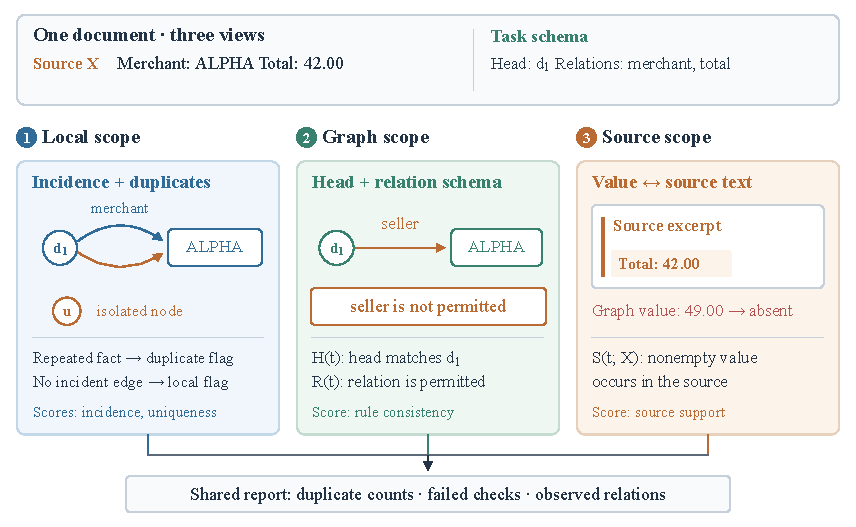
\includegraphics[width=0.98\textwidth]{figure/method/image2.pdf}
    \caption{Three scopes of graph checks. Local checks find repeated facts
and unlinked nodes. Graph checks test document IDs and field names.
Source checks look for values in the text. Both repair paths use these
groups to build an assessment profile.}
    \label{fig:scale_relationship}
\end{figure}

Cleanup first fixes errors with clear rule-based changes.
The preprocessor $P$ removes duplicate triples.
It reverses an edge if its object is $h_0$ and its subject is a different node.
It then removes triples with an invalid head or relation.
Here, the head is the subject of a triple.
The cleaned graph is $G_s=P(G;h_0,\mathcal R_X)$.

For a triple $t=(h,r,o)$, the three checks are
\begin{equation}
    \label{eq:diagnostic_predicates}
    H(t)=\mathbf1[h=h_0],\quad
    R(t)=\mathbf1[r\in\mathcal R_X],\quad
    S(t;X)=\mathbf1[o\ne\emptyset\ \wedge\ o\text{ occurs in }X].
\end{equation}
$H$ checks the document ID, $R$ checks the relation, and $S$ checks the source.
Keeping these checks separate gives a reason for each rejected triple.

The main path uses an assessment profile in the form of an error report:
\begin{equation}
    \label{eq:diagnostic_context}
    D(G_s,X)=\big(n_{\mathrm{dup}},I_H,I_R,I_S,\mathcal R(G_s)\big).
\end{equation}
The report stores duplicate counts, failed-check positions, and present relations.
For example, $I_S=\{i:S(t_i;X)=0\}$ lists positions that fail the source check.
The report uses the cleaned input.
It tells the model where to look when proposing field values.
We test the effect of adding this report to the prompt.
Fields are optional, and the main path calls the model once per document.

\subsection{Generating a Graph from Source Text}
\label{sec:framework:architecture}

Rules fix clear structural errors; a language model reads values from the text.
It returns an ordered list of triples:
\begin{equation}
    \label{eq:proposal_generation}
    C=L_\theta(X,h_0,\mathcal R_X,G_s,D(G_s,X)).
\end{equation}
The prompt asks for a complete graph.
It tells the model to copy source values, keep correct fields, and fill missing
or wrong values.
The JSON parser returns an empty graph for an invalid response.
Scoring includes these empty graphs.
The base prompt uses the same inputs and output limit, with the report removed.

\subsection{Checking the Generated Triples}
\label{sec:framework:constraints}

Constraints decide which proposed triples enter the repaired graph.
The gate is a filter that keeps source-matched values under the allowed fields.
It also keeps at most one value per relation.
Let $\operatorname{uniq}(C)$ remove copies in output order.
The triples that pass the checks are
\begin{equation}
    \label{eq:eligible_candidates}
    C_X=\{t\in\operatorname{uniq}(C):H(t)R(t)S(t;X)=1\}.
\end{equation}
The allowed output sets are
\begin{equation}
    \label{eq:admissible_subsets}
    \mathcal F(C_X)=\left\{A\subseteq C_X:
    \sum_{t\in A}\mathbf1[r_t=r]\leq1,\ \forall r\in\mathcal R_X\right\}.
\end{equation}
Equation~\ref{eq:eligible_candidates} sets the evidence and schema requirements.
Equation~\ref{eq:admissible_subsets} sets the field-count limit.
Together, they define which outputs the filter can keep.

The filter scans candidates in order and keeps the first valid value per field.
The output $\widehat G$ has size
\begin{equation}
    \label{eq:selection_size}
    |\widehat G|=\max_{A\in\mathcal F(C_X)}|A|
    =|\{r:\exists t\in C_X,\ r_t=r\}|.
\end{equation}
Each field forms one group with room for one triple.
The filter keeps one triple from every group with a valid candidate.
It thus keeps the largest allowed number of candidates.
Output order breaks ties between values that pass the same checks.

\subsection{Field Meanings and Source Lines}
\label{sec:framework:field_evidence}

Source evidence also helps the model choose between nearby values.
A receipt can list a brand, a company, a subtotal, and a final amount.
We give each field a short meaning to guide this choice.
All receipt repair methods receive these meanings and numbered source lines.

The source-line index adds hints for each field.
Fixed patterns find company terms, address terms, postcodes, dates, and total labels.
Each matching line is an anchor.
The index includes that line, one line before it, and two lines after it.
Simple receives the full source and field meanings.
Evidence Index also receives the line hints.

The receipt filter uses the same whitespace rule as the parser.
$N(s)$ changes each run of spaces or line breaks to one space and trims the ends.
The source check is
\begin{equation}
    S_{\mathrm{ws}}(t;X)=\mathbf1[|N(o)|>0\ \wedge\
    N(o)\text{ occurs in }N(X)].
\end{equation}
It keeps word boundaries, case, and punctuation.
The receipt follow-up uses this check.
Earlier tests use the original exact-text check.

\section{Implementation}
\label{sec:implementation}

The implementation turns the checks into repair steps.
Section~\ref{sec:impl:assessment} gives the main generation-and-filter path.
Sections~\ref{sec:impl:optimizer_audit} and~\ref{sec:method:algorithm}
give the separately tested edit-selection path.

\subsection{Repair Steps}
\label{sec:impl:assessment}

Algorithm~\ref{alg:abstract} gives Diagnosis + Gate.
Diagnosis is the error report. Gate is the triple filter.
Code builds the report and runs the checks.
The model proposes field values.
The filter returns the repaired graph and a rejection log.

\begin{algorithm}[t]
\caption{Repair with source text and field checks}
\label{alg:abstract}
\begin{algorithmic}[1]
\Require Input triples $G$, source $X$, document ID $h_0$, allowed relations $\mathcal R_X$
\Ensure Repaired graph $\widehat G$ and rejection log $J$
\State $G_s\gets P(G;h_0,\mathcal R_X)$
\State $D\gets D(G_s,X)$
\State $C\gets\textsc{Parse}(L_\theta(X,h_0,\mathcal R_X,G_s,D))$
\State $\widehat G\gets\emptyset$; $J\gets\emptyset$; $B\gets\emptyset$
\For{each candidate $t=(h,r,o)$ in generation order}
    \If{$t$ appeared earlier in $C$}
        \State append $(t,\text{duplicate})$ to $J$
    \ElsIf{$H(t)R(t)S(t;X)=1$ and $r\notin B$}
        \State $\widehat G\gets\widehat G\cup\{t\}$; $B\gets B\cup\{r\}$
    \Else
        \State append $(t,\text{failed check})$ to $J$
    \EndIf
\EndFor
\State \Return $\widehat G,J$
\end{algorithmic}
\end{algorithm}

The runner passes the source, document ID, allowed relations, and input triples
to the model.
The scorer loads the reference values.
Tests change references and defect labels and check that model inputs stay the same.
The older loader reads the document ID from the reference record as task information.

With hash-based lookups, cleanup takes $O(|G|)$ triple operations on average.
Filtering $k$ candidates costs $O(k(1+c_X))$ and uses
$O(k+|\mathcal R_X|)$ extra memory.
Here, $c_X$ is the cost of finding a value in the text.
Text length affects this cost.
We time model calls apart from these checks.

\subsection{Prompt and Rule Settings}
\label{sec:impl:enhancement}

\subsubsection{Shared Prompts and Responses}

One system prompt supports three settings: basic input, an error report,
and SHACL checks.
Three calls give three responses for each input.
We score each response before and after filtering, giving six scores.
Each before/after pair uses the same triples.
This keeps candidate generation fixed when measuring the filter.

The model is \texttt{google/gemma-4-26B-A4B-it} at temperature zero.
The output limit is 4,000 tokens in each setting.
We report input tokens because prompt lengths differ.
Request times include retries and pacing waits.
We save all responses and score invalid responses too.
The earlier Claude tests use a separate prompt for each method.

\subsubsection{SHACL Prompt Baseline}
\label{sec:impl:shacl}

Lin et al.\ use five prompt parts: an introduction, detected errors,
SHACL rules, graph context, and instructions \citep{ref_lin2025}.
We use their full-rules/full-graph ($M+G$) setting for the field task.
The pySHACL tool checks document IDs, allowed relations, nonempty values,
and field counts.
A SPARQL rule checks values against the source text.

The prompt includes the full source and returns a complete JSON graph.
It groups each document's errors into one call.
We call this baseline \emph{Lin-style SHACL context (adapted)}.
RDF stores unique triples.
Our shared JSON input keeps duplicate copies.
We score the output before and after filtering for each prompt setting.

\subsection{Scale-Aware Routing and Edit Actions}
\label{sec:impl:optimizer_audit}
\label{sec:method:decision}

An edit selector must decide which part of the graph to change next.
Several edits may target the same field or undo another edit.
The selector uses the assessment profile to weigh these choices.
Scale-aware routing gives weights to local, graph, and source-based edits.
Trial checks then compare their gains and costs.
Figure~\ref{fig:framework_overview} shows this path.

\begin{figure}[t]
    \centering
    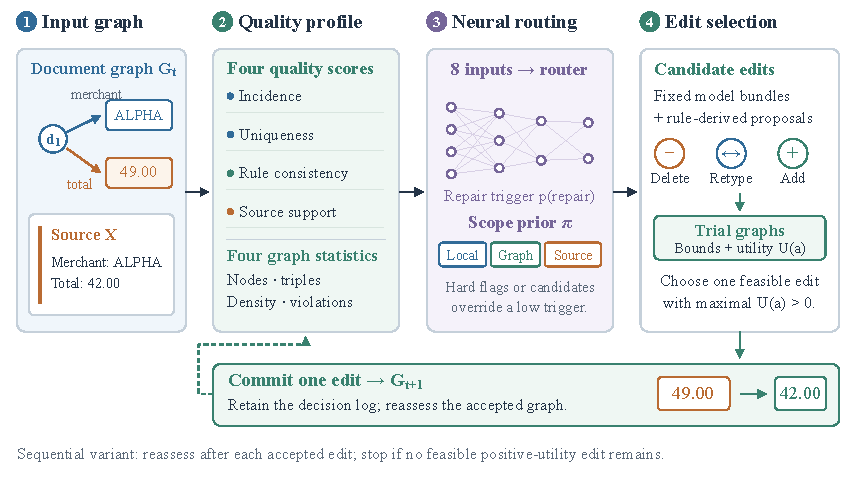
\includegraphics[width=0.98\textwidth]{figure/method/image1.pdf}
    \caption{Scale-aware routing for edit selection. The assessment profile
and graph counts feed the router. It gives a repair score and weights for
three edit scopes. The selector tries model and rule edits on graph copies,
applies the best allowed positive-score edit, and checks again.}
    \label{fig:framework_overview}
\end{figure}

\subsubsection{Assessment Profile and Shared Inputs}
\label{sec:impl:profile_revision}

The selector's assessment profile uses four scores.
They measure linked nodes, unique triples, rule agreement, and source support:
\begin{equation}
\label{eq:quality_state}
\begin{split}
\mathbf{s}={}&(Q_{\mathrm{inc}},Q_{\mathrm{uniq}},Q_{\mathrm{rule}},Q_{\mathrm{src}}),\\
Q_i={}&100(1-r_i),\quad Q=\tfrac14\sum_i Q_i.
\end{split}
\end{equation}
Each $r_i$ is an error rate for its check.
For a nonempty graph, the rates are
\begin{equation}
\label{eq:profile_rates}
r_{\mathrm{inc}}=\frac{I}{n},\quad
r_{\mathrm{uniq}}=\frac{m-c}{m},\quad
r_{\mathrm{rule}}=\frac{B}{m},\quad
r_{\mathrm{src}}=\frac{V}{m}.
\end{equation}
$I$ counts unlinked nodes, and $c$ counts triple similarity groups.
$B$ counts distinct triples flagged by graph rules.
$V$ counts values absent from the text after removing whitespace.
Here, $n$ and $m$ count nodes and triples.
These scores give a common scale for comparing trial graphs.
An empty graph has node-link score zero and the other three scores 100.
For a nonempty graph without source text, the source score is 50.

Triple similarity uses character-pair counts for the subject, relation, and value.
Their cosine similarities have weights 0.4, 0.2, and 0.4.
Pairs at or above 0.92 form groups for the uniqueness score.
Hierarchy checks use management, supervision, and membership directions.
They skip relations with unclear meanings.
Entity checks apply to endpoints marked as entity references.
Other field values are treated as text.

The profile also reports missing source fields.
The source-field check reads values after allowed labels at a document,
line, or sentence start.
It adds a candidate when the text gives a field that the graph omits.
It skips a field when repeated labels give conflicting values.
These reports enter the violation count and candidate list.

The router receives four scores and four graph counts:
\begin{equation}
\label{eq:routing_inputs}
\mathbf{g}=(n,m,\rho,n_{\mathrm{viol}}),\qquad
\rho=\frac{|E_{\mathrm{pair}}|}{n(n-1)}\quad(n>1).
\end{equation}
Here, $n$ and $m$ count nodes and triples.
$E_{\mathrm{pair}}$ contains distinct directed node pairs without self-links.
Density is zero when $n\leq1$.
$n_{\mathrm{viol}}$ counts the reported violations.
The main report $D$ lists field errors; $\mathbf{s}$ scores the selector's graph.
Both are forms of the assessment profile, used by their respective repair paths.

\subsubsection{Router and Training Signals}

The router turns these eight inputs into a repair score and scope weights:
\begin{equation}
\label{eq:decision_net}
(p_{\mathrm{repair}},\boldsymbol{\pi})=
f_\phi(\operatorname{scale}([\mathbf{s};\mathbf{g}])).
\end{equation}
$\operatorname{scale}$ uses training-set means and standard deviations.
$\boldsymbol{\pi}$ has three nonnegative weights that sum to one.
They weigh entity, graph, and context edits.
The network has layers of size $8\!\rightarrow\!32\!\rightarrow\!16$,
one repair output, and three scope outputs: 884 parameters in all.
Both hidden layers use ReLU.
A sigmoid gives the repair score, and a softmax gives the scope weights.
Training and use share the same feature code.
A feature-version mismatch switches the router to equal weights.

Training labels come from the known added defects.
The repair label $y_j$ is one for a degraded graph and zero for its clean pair.
The scope label $c_j$ is the most frequent defect scope in that graph.
Clean graphs train the repair output only.
The loss is
\begin{equation}
\label{eq:decision_loss}
\begin{split}
\mathcal L(\phi)={}&\frac1N\sum_j\operatorname{BCE}(p_j,y_j)\\
&+\frac{\sum_j b_j(-\log\pi_{j,c_j})}{\sum_j b_j+\epsilon}.
\end{split}
\end{equation}
$b_j$ is one when a scope label is present, and $\epsilon$ avoids division by zero.
The first term trains the repair score.
The second trains the scope weights on degraded graphs.
Document groups stay within one training, validation, or test split.
The selector uses task inputs and source text to compute its features.

\subsubsection{Candidate Edits and Costs}
\label{sec:method:modalities}

Rules and model proposals provide candidate edits.
The selector can delete a triple, change its relation, or add a triple.
The relation-change operation is called retype in the code.
Related edits can form one bundle.
In the saved-proposal test, changes between the cleaned input and model output
are grouped by relation.
Each group is a bundle with confidence 0.7.

Edit costs favor small changes:
\begin{equation}
\label{eq:cost_hierarchy}
c(a)=\begin{cases}
0.30 & \text{delete},\\
0.16 & \text{retype},\\
0.06 & \text{add}.
\end{cases}
\end{equation}
A bundle's cost is the sum of its edit costs.
These fixed costs enter the trial score along with quality gain and scope weights.
The learned-prior test compares the router with an always-on equal-weight prior.

\subsection{Trial Checks and Repair Loop}
\label{sec:method:algorithm}

Each candidate is tried on a graph copy before any edit is committed.
Let $G_a$ be the trial graph, $h$ the hard-rule error count,
$\sigma(a)$ the edit scope, and $z(a)$ its confidence.
The default score is
\begin{equation}
\label{eq:action_utility}
\begin{split}
U(a)={}&\frac{Q(G_a)-Q(G)}{100}
+0.20\frac{\max(0,h(G)-h(G_a))}{\max(1,h(G))}\\
&-0.35c(a)+0.05\log\!\left(\max(\pi_{\sigma(a)},0.05)+10^{-6}\right)
+0.02z(a).
\end{split}
\end{equation}
The terms measure quality gain, fewer rule errors, edit cost, scope weight,
and candidate confidence.
The trial recomputes the full graph profile.
It also checks score bounds, density, and whether an edit would empty the graph.

The score lower bounds are 55, 55, 60, and 45 for the four profile scores.
An already met bound stays met.
A score below its bound must stay the same or increase.
Each checked score can fall by at most two points, subject to these bounds.
Trial density is at most 0.75.
A nonempty graph stays nonempty.
These requirements define the allowed trial set $\mathcal A_t^{\mathrm{ok}}$.
The selection step is
\begin{equation}
\label{eq:constrained_opt}
a_t^*=\arg\max_{a\in\mathcal A_t^{\mathrm{ok}}}U(a),\qquad U(a_t^*)>0.
\end{equation}
Equation~\ref{eq:constrained_opt} chooses among the current trial edits.
The bounds decide which edits are allowed; the score orders the allowed edits.
The graph stays unchanged when no allowed edit has a positive score.

\begin{figure}[t]
    \centering
    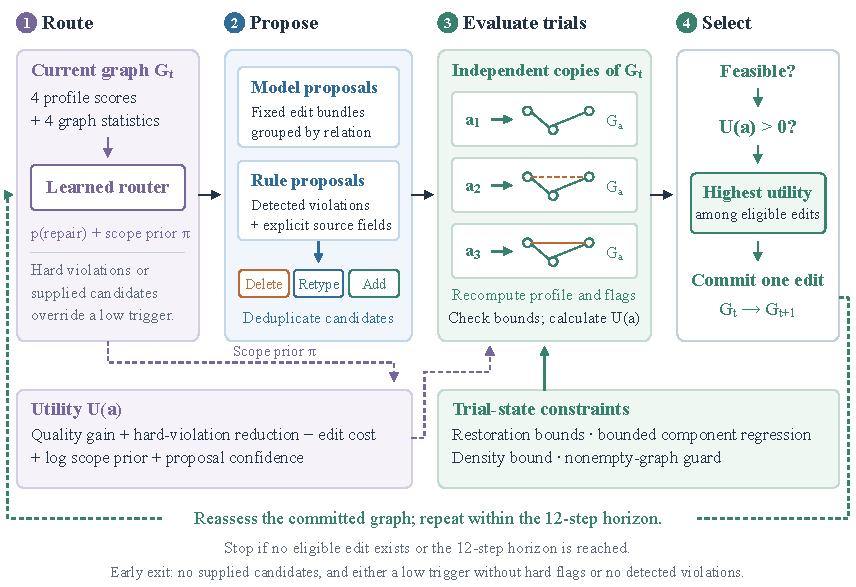
\includegraphics[width=0.98\textwidth]{figure/method/image3.pdf}
    \caption{One round of trial checking. The router weighs edit scopes.
The selector scores each model or rule edit on a graph copy, checks the
bounds, and applies the best allowed positive-score edit. It then rebuilds
the assessment profile. The saved-proposal test allows twelve rounds.}
    \label{fig:optimization_flow}
\end{figure}

Algorithm~\ref{alg:enhancement} links assessment, routing, and execution.
Supplied candidates or hard-rule errors start trial checks even with a low
repair score.
The loop ends when no useful allowed edit remains, no trial is needed,
or the step limit is reached.
Logs save trial graphs, scores, decisions, and stop reasons.

\begin{algorithm}[t]
\caption{Scale-aware edit selection with trial checks}
\label{alg:enhancement}
\begin{algorithmic}[1]
\Require Input graph $G$, source $X$, supplied candidates $A_0$, task inputs, step limit $T$
\Ensure Repaired graph $\widehat G$ and decision log $J$
\State $\widehat G\gets G$; $J\gets\emptyset$; $E\gets\emptyset$
\State add missing source-field candidates to $A_0$
\For{$t=1$ to $T$}
    \State compute profile and $(p_{\mathrm{repair}},\boldsymbol\pi)$ for $\widehat G$
    \If{$A_0=\emptyset$, $h(\widehat G)=0$, and $p_{\mathrm{repair}}<\tau_{\mathrm{repair}}$}
        \State \textbf{break}
    \EndIf
    \If{no reported violations and $A_0=\emptyset$}
        \State \textbf{break}
    \EndIf
    \State $A\gets\textsc{Unique}(A_0\cup\textsc{RuleEdits}(\widehat G))$
    \State skip graph--candidate pairs already in $E$
    \State try each remaining $a\in A$ on a copy and record its pair in $E$
    \State check graph bounds and compute $U(a)$ for each trial
    \State append trial scores and decisions to $J$
    \If{no allowed candidate has $U(a)>0$}
        \State \textbf{break}
    \EndIf
    \State apply the allowed edit with the highest $U(a)$ to $\widehat G$
\EndFor
\State \Return $\widehat G,J$
\end{algorithmic}
\end{algorithm}

The saved-proposal test uses $T=12$ and $\tau_{\mathrm{repair}}=0.05$.
A second score subtracts $0.05\log(1/3+10^{-6})$ from the default score.
This sets the prior term to zero for equal weights.
It keeps the edit order for a fixed router but shifts the positive-score cutoff.
Both scores are fixed before the saved-proposal tests.
Source matching in this selector removes whitespace from both strings.
The archive also stores earlier logs with separate whitespace rules.
Algorithm~\ref{alg:abstract} and the selector have separate tests.

Pairwise triple checks cost $O(m^2)$ for $m$ triples.
$T$ rounds with up to $K$ trials per round cost $O(TKm^2)$, plus text checks.
The main filter scans the candidate list once.
